\subsection{Numerical Integration Methods - Chapter 25}

\begin{enumerate}

\item {\bf Truncation Error in Euler's Method}

  The inherent problem associated with Euler's method is the
  assumption that the derivative is linear in between the interval
  $\Delta t$. That is, Euler's method assumes the slope $\dot{f}_1$ is
  constant over time 1 to 2.

  \begin{equation}
    f_2 \approx f_1 + \dot{f}_1\Delta t 
  \end{equation}

  However, the taylor series expansion clearly states that f can be
  approximated as an expansion of multiple terms. The equation below
  is the taylor series expansion starting at $f(t_0)$.

  \begin{equation}
    f(t_1) \approx f(t_0) + \dot{f}(t_0)\Delta t +
    \frac{\ddot{f}(t_0)}{2!}\Delta t^2 + ... + \frac{f^{(N)}(t_0)}{N!}\Delta t^N
  \end{equation}

  Notice that Euler's method is merely the first two terms. Thus we
  can write that the error accrued by Euler's method is

  \begin{equation}
    E_{T} = \frac{\ddot{f}(t_0)}{2!}\Delta t^2 + ... + \frac{f^{(N)}(t_0)}{N!}\Delta t^N
  \end{equation}

  This type of error is called Truncation Error and is a direct result
  of truncating the higher order terms (HOTs) in the taylor series
  expansion. 

\item {\bf Taylor Series Approximation to Euler's Method}

  Note however, that it is extremely easy to include higher order
  terms in Euler's method. That is we can simply include three terms
  instead of just two and suddenly Euler's method becomes second
  order.

  \begin{equation}
    f(t_{i+1}) \approx f(t_i) + \dot{f}(t_i)\Delta t +
    \frac{\ddot{f}(t_i)}{2!}\Delta t^2
  \end{equation}

  The issue with this method is that the second derivative must be
  know. Often this derivative is not known and the method cannot be
  used. To mitigate this a class of higher order methods is typically used.

\item {\bf Heun's Method}

Heun's method is derived such that $p_1=1$, $q_{11} = 1$, and $a_1 =
a_2 = 1/2$. Heun's method is then given using the equation below.

\begin{equation}
\begin{matrix}
y_{k+1} = y_k + \phi \Delta t \\
\phi = \frac{1} 2(k_1 + k_2) \\
k_1 = f(t_k,y_k) \\
k_2 = f(t_k + \Delta t,y_k + k_1 \Delta t) \\
\dot{y} = f(t,y)
\end{matrix}
\end{equation}

This can also be represented graphically as shown below.

\begin{figure}[H]
  \begin{center}
    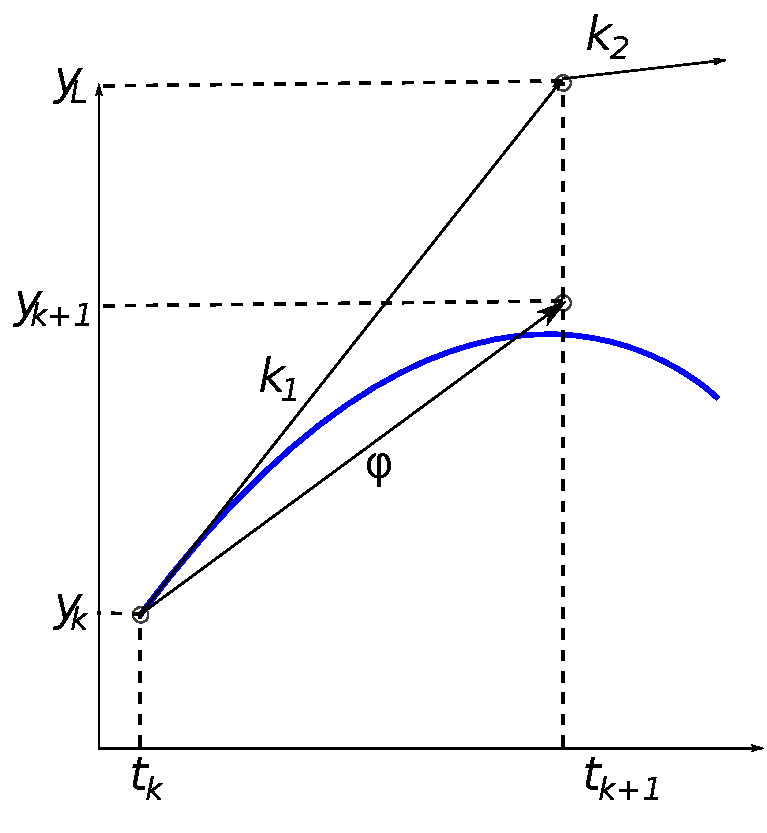
\includegraphics[height=0.6\textwidth,width=0.62\textwidth]{Graphics/Heuns_Method.pdf}
  \end{center}
\end{figure}

\item {\bf Runge-Kutta}

Runge-Kutta techniques are a class of higher order integration
methods. They all have the same form using the equation below.

\begin{equation}
\begin{matrix}
y_{k+1} = y_k + \phi \Delta t \\
\phi = a_1 k_1 + a_2 k_2 + ... + a_n k_n \\
k_1 = f(t_k,y_k) \\
k_2 = f(t_k + p_1 \Delta t,y_k + q_{11} k_1 \Delta t) \\
k_3 = f(t_k + p_2 \Delta t,y_k + q_{21}k_1 \Delta t +
q_{22}k_2\Delta t) \\
\vdots \\
k_n = f(t_k + p_n \Delta t,y_k + q_{n1}k_1 + ... q_{nn}k_{n-1}) \\
\dot{y} = f(t,y)
\end{matrix}
\end{equation}

The coefficients $a_n$ and $q_n$ must be solved using the taylor
series expansion. The number $n$ is the order of the method. Thus if
$n=2$ the order of the method is quadratic and is called an RK2
technique.

\item {\bf Runge-Kutta-4}

The Runge-Kutta-4 (RK4) algorithm is the standard in numerical
simulations. This method uses 4 function calls and is computed using
the equation below.

\begin{equation}
\begin{matrix}
y_{k+1} = y_k + \phi \Delta t \\
\phi = \frac{1} 6(k_1 + 2 k_2 + 2 k_3 + k_4) \\
k_1 = f(t_k,y_k) \\
k_2 = f(t_k + \Delta t/2,y_k + k_1 \Delta t/2) \\
k_3 = f(t_k + \Delta t/2,y_k + k_2 \Delta t/2) \\
k_4 = f(t_k + \Delta t,y_k + k_3 \Delta t) \\
\dot{y} = f(t,y)
\end{matrix}
\end{equation}

Again, the RK4 method can be represented graphically as shown below.

\begin{figure}[H]
  \begin{center}
    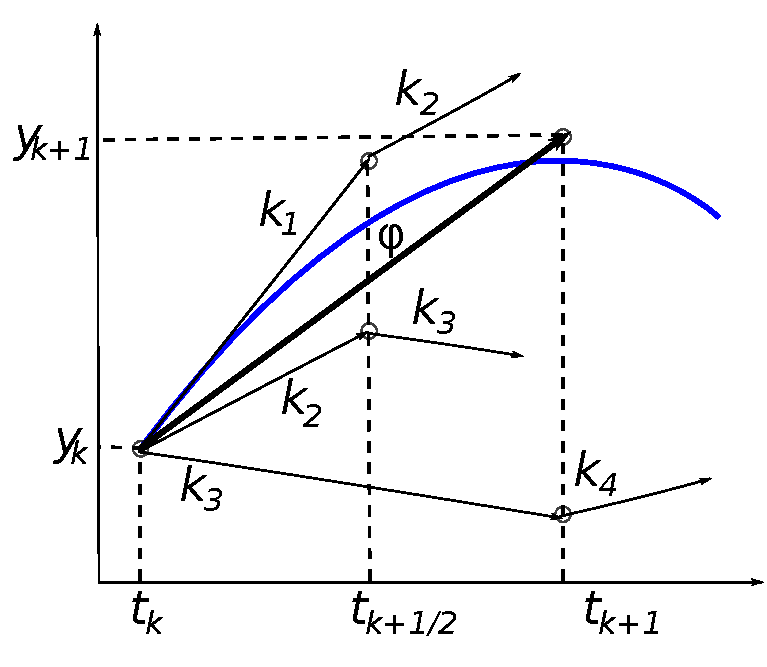
\includegraphics[height=0.55\textwidth,width=0.6\textwidth]{Graphics/RK4.pdf}
  \end{center}
\end{figure}

\item {\bf Shower Problem}
  
  Let's return to our shower problem from the bi-section method except
  this time we want to model the rise in temperature as a function of
  time. Let's assume the problem is first order as shown below where

  \beq
  \dot{T} + \tau T = \tau T_c
  \eeq

  where $\tau$ is a time constant and $T_c$ is a commanded
  temperature. Again the solution to this equation is simple and can
  be determined using differential equation techniques to achieve the
  solution below

  \beq
  T(t) = T_0e^{-\tau t} + T_c(1-e^{-\tau t})
  \eeq

  The solution to this equation is shown below. Notice the rise time
  in the graph here which is dictated by $\tau$. 

  \begin{figure}[H]
    \begin{center}
      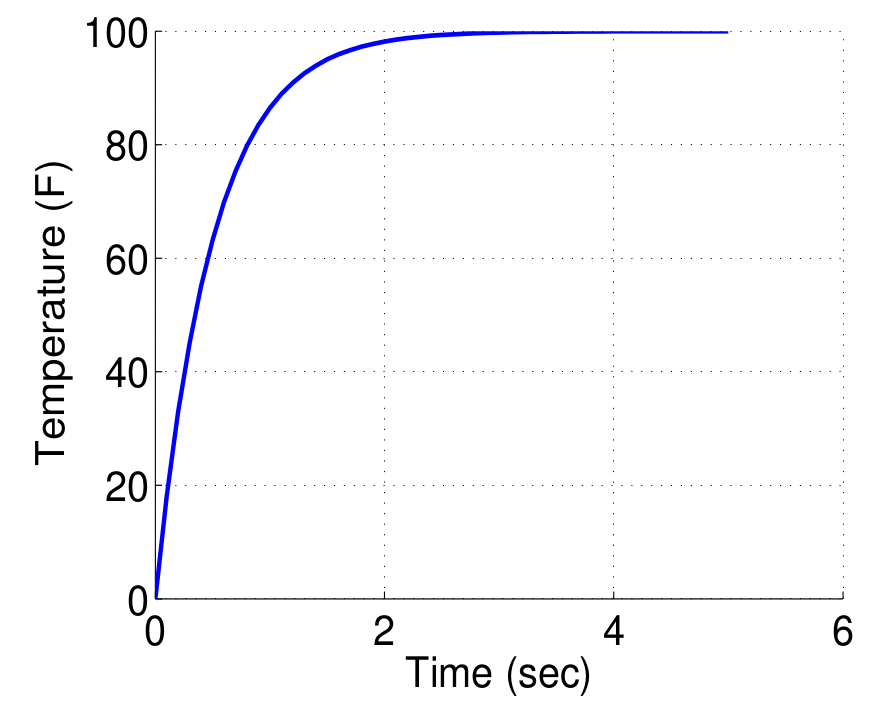
\includegraphics[height=0.4\textwidth,width=0.5\textwidth]{Graphics/Temp_Eulers}
    \end{center}
  \end{figure}

  Now what if we make the problem a bit more complex and let $T_c =
  k\theta$ where $\theta$ is the angle of the shower knob. This would
  mean our equations of motion become

  \beq
  \dot{T} + \tau T = \tau k \theta
  \eeq

  So what's $\theta$? Well we would like to turn the knob bigger when
  the water is too cold and turn it down when the water is too
  hot. Something like this

  \beq
  \theta_{n+1} = \begin{Bmatrix} \theta_n + 2,T<T_c
    \\ \theta_n-2,T>T_c\end{Bmatrix}
  \eeq

  So if the water is too cold we turn the knob 2 degrees and if it's
  too hot we turn it down 2 degree. To make it more complicated we
  only check every 5 seconds and if the water is within 5 degrees we
  stop changing the temperature. So what does that analytic
  solution look like? Well this would require Euler's method or
  RK4. Let's do Euler's method first, let $\theta_0 = 0~deg$, $k = 5~F/deg$, $\tau
   = 2~/sec$ and $T_0 = 0$ and $\Delta t = 0.1~s$. Let, $T_c = 100~F$.

  \beq
  \begin{matrix}
  \dot{T}_0 = \tau k \theta_0 - \tau T_0\\
  T_1 = T_0 + \dot{T}_0 \Delta t\\
  \dot{T}_1 = \tau k \theta_1 - \tau T_1\\
  T_2 = T_1 + \dot{T}_1 \Delta t\\
  \vdots\\
  \dot{T}_N = \tau k \theta_N - \tau T_N\\
  T_{N+1} = T_N + \dot{T}_N \Delta t\\
  \end{matrix}
  \eeq

  The code for this is a bit more complex but it's left out as an
  exercise. If the timestep is sufficiently small (0.1 seconds) Euler's method will
  converge to the solution and produce the result below. 

  \begin{figure}[H]
    \begin{center}
      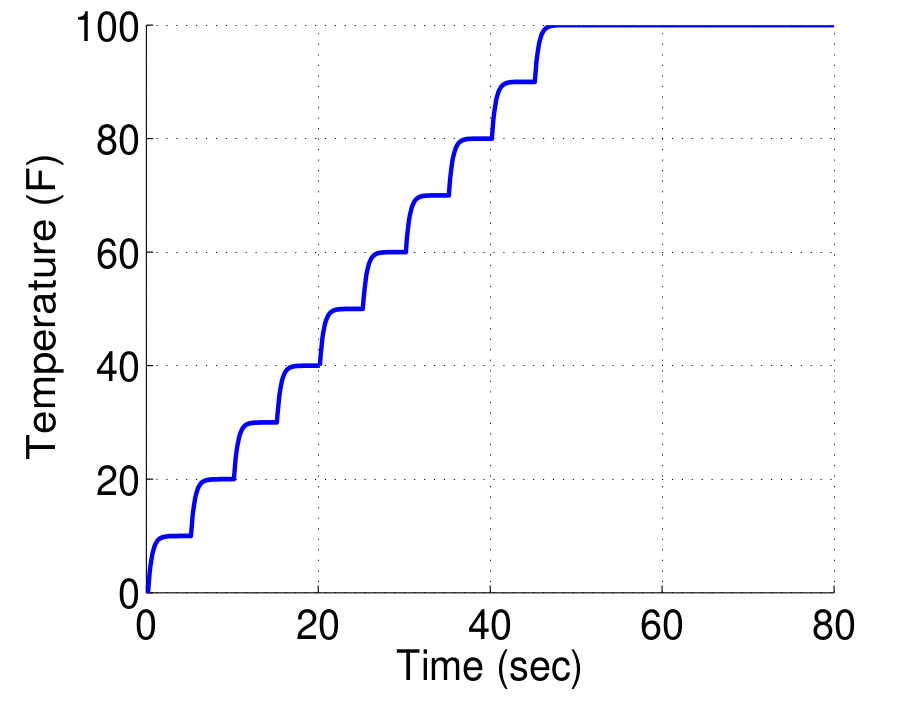
\includegraphics[height=0.4\textwidth,width=0.5\textwidth]{Graphics/Euler_Feedback}
    \end{center}
  \end{figure}

  Notice that every 5 seconds we turn up the temperature until we
  arrive at 100 degrees. You can see that this doesn't really have an
  analytical solution. We can then do the same thing for the Runge
  Kutta Method. Here our iterative method becomes

  \beq
  \begin{matrix}
  k_1 = \tau k \theta - \tau T_0\\
  k_2 = \tau k \theta - \tau (T_0 + k_1\Delta t/2)\\
  k_3 = \tau k \theta - \tau (T_0 + k_2\Delta t/2)\\
  k_4 = \tau k \theta - \tau (T_0 + k_3\Delta t)\\
  \phi = (1/6)(k_1 + 2k_2 + 2k_3 + k_4)\\
  T_1 = T_0 + \phi \Delta t\\
  \vdots
  \end{matrix}
  \eeq

  The solution using the iterative method above is the same the
  difference is that we can increase the timestep and still get good
  results. The figure below shows the solution using Euler's and RK4
  using a much larger timestep (0.8 seconds). Notice that RK4 still converges
  and Euler's method begins to have abnormal oscillations.
  
  \begin{figure}[H]
    \begin{center}
      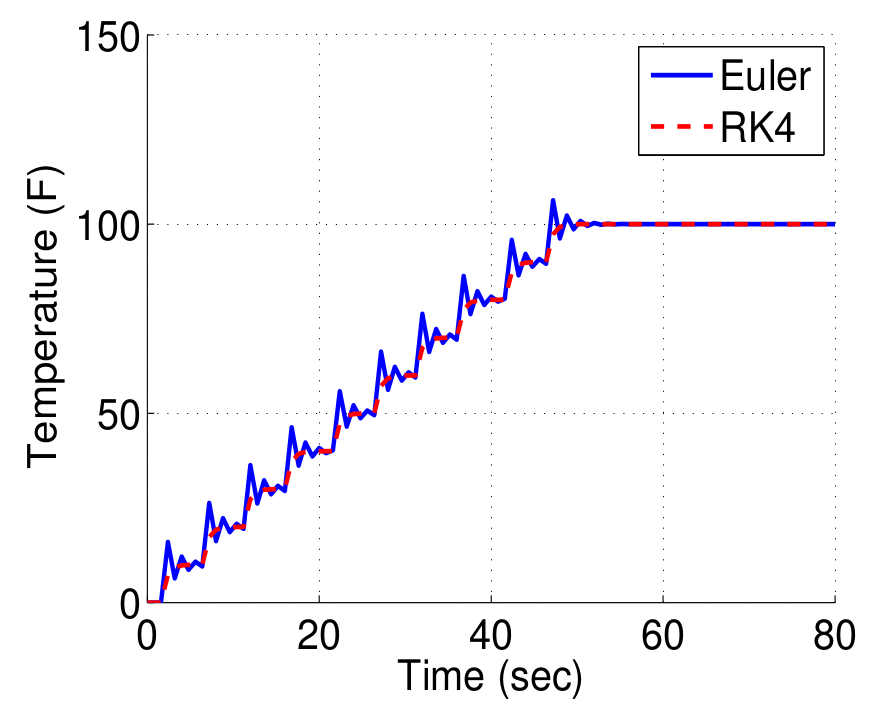
\includegraphics[height=0.4\textwidth,width=0.5\textwidth]{Graphics/Euler_RK4}
    \end{center}
  \end{figure}

  \item {\bf Camera Tracker}

    Assume you'd like to track a moving target. We will restrict
    ourselves to a ball being launched vertically such that $z(t) =
    z_0 + v_0t - 0.5gt^2$. The camera is always pointed towards the
    object but requires an elevation angle command. 

    \beq
    \theta_c = tan^{-1}(z/x_s)
    \eeq

    where $x_s$ is the horizontal distance from the camera and the
    ball. Let's let the dynamics of the elevation angle be determined
    using the equation below

    \beq
    \ddot{\theta} = \frac{T-c\dot{\theta}}{J}
    \eeq

    where $J$ is the moment of inertia of the camera and $c$ is a
    friction coefficient which models the bearing the camera sits
    on. In order to track the object properly we need to apply
    proportional feedback control such that

    \beq
    T = -k_p(\theta-\theta_c)
    \eeq

    Thus our equation of motion becomes

    \beq
    \ddot{\theta} = \frac{-k_p(\theta-\theta_c)-c\dot{\theta}}{J}
    \eeq

    Again, if $\theta_c$ is a constant the solution becomes 

    \beq
    \theta(t) = (\alpha_1 cos(\omega t) + \alpha_2 sin(\omega
    t))e^{\sigma t} + \theta_C
    \eeq
    
    where $\alpha_1$ and $\alpha_2$ are determined using initial
    conditions and $\sigma \pm \omega i$ is the solution to the
    characteristic equation when solving the differential
    equation. If $\theta_0 = \dot{\theta}_0 = z_0 = 0$, $v_0 = 20~m/s$,
    $J = 0.1 kg-m^2$, $k_p=20$, $c = 1$, $x_s = 40~m$, and $\theta_c =
    45 degrees$ the analytic solution is shown below. 

    \begin{figure}[H]
      \begin{center}
        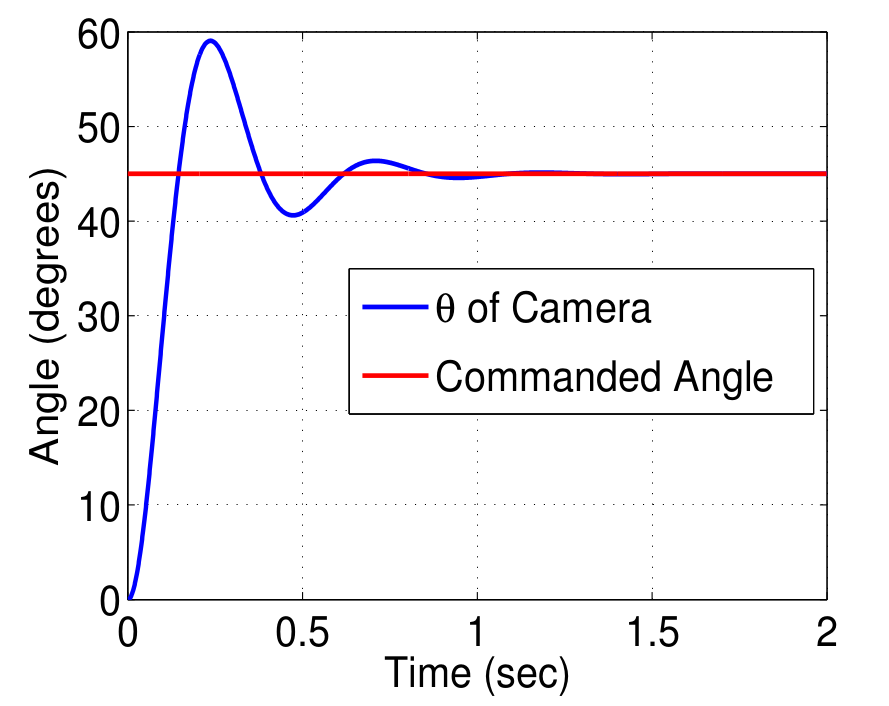
\includegraphics[height=0.4\textwidth,width=0.5\textwidth]{Graphics/Camera_Track_Constant}
      \end{center}
    \end{figure}
    
    It looks like our camera over shoots by a bit but that dynamics
    can be tuned easily in our simulation to obtain the desired
    response. Now, if $\theta_C$ is not constant the solution is not
    analytic and the solution must be obtained numerically. The
    easiest way to solve this system of equations numerically is to
    put the equation in first order form. To do this we set
    $x_1=\theta$ and $x_2 = \dot{\theta}$. Thus $\dot{x}_1 =
    \dot{\theta} = x_2$ and $\dot{x}_2 = \ddot{\theta} =
    -c\dot{\theta}/J-k_p(\theta-\theta_c)/J = -c x_2/J -
    k_p(x_1-\theta_c)/J$. This can be put in matrix form to yield the
    equation below

    \beq
    \begin{Bmatrix} \dot{x}_1 \\ \dot{x}_2 \end{Bmatrix}
    = \begin{bmatrix} 0 & 1 \\ -k_p/J &
      -c/J \end{bmatrix}\begin{Bmatrix}x_1 \\ x_2 \end{Bmatrix}
    + \begin{Bmatrix}0 \\ k_p/J \end{Bmatrix} \theta_c
    \eeq

    This can be written in more compact form as $\vec{\dot{x}} =
    A\vec{x} + Bu$ where $A$ and $B$ are matrices. The great thing
    about this equation is that the solution to this equation if $u=0$
    is simply $\vec{x}(t) = e^{At}\vec{x}_0$ where $\vec{x}_0$ is the
    initial condition vector. If this matrix form is used for Euler's
    method the iterative sequence becomes

    \beq
    \begin{matrix}
    \dot{x}_0 = A x_0 + B u_0 \\
    x_1 = x_0 + \dot{x_0} \Delta t\\
    \dot{x}_1 = A x_1 + B u_1 \\
    x_2 = x_1 + \dot{x_1} \Delta t\\
    \vdots\\
    \dot{x}_N = A x_N + B u_N \\
    x_{N+1} = x_N + \dot{x_N} \Delta t\\
    \end{matrix}
    \eeq

    hence why the matrix form equation is so powerful. The $A$ and $B$
    matrices are constant and thus the iterative method is extremely
    simple. If the iterative method is used to compute the solution
    where $\theta_c$ is not constant the solution can be seen in the
    figure below.

    \begin{figure}[H]
      \begin{center}
        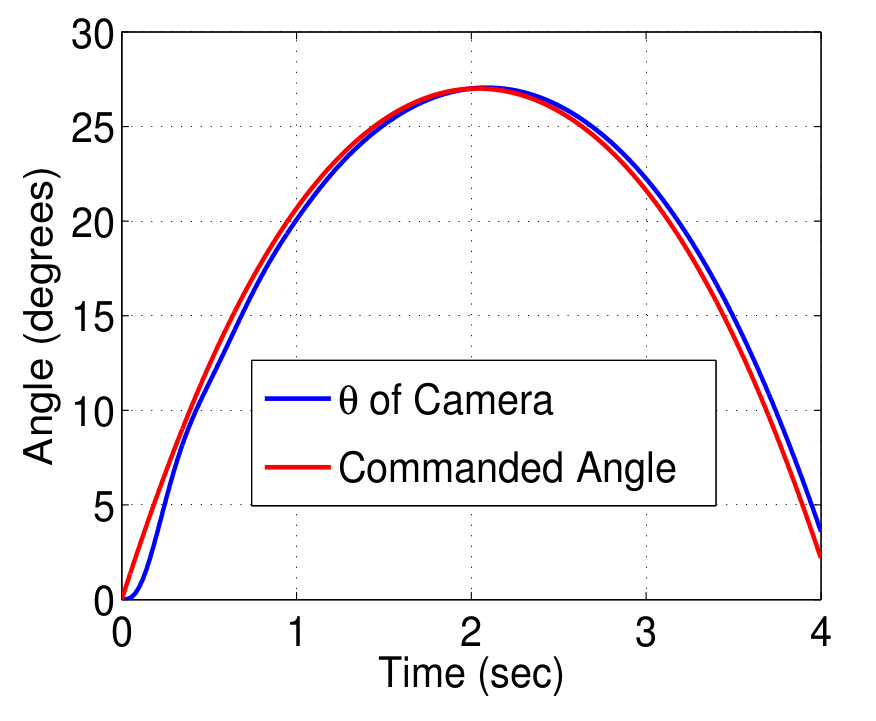
\includegraphics[height=0.4\textwidth,width=0.5\textwidth]{Graphics/Camera_Tracking_Active}
      \end{center}
    \end{figure}

    Notice the slight lag in the camera which is just a product of
    active feedback. 
    
\end{enumerate}
